\documentclass[12pt,a4paper]{article}
\usepackage{geometry}
\geometry{left=2.5cm,right=2.5cm,top=2.0cm,bottom=2.5cm}
\usepackage[english]{babel}
\usepackage{amsmath,amsthm}
\usepackage{amsfonts}
\usepackage[longend,ruled,linesnumbered]{algorithm2e}
\usepackage{fancyhdr}
\usepackage{ctex}
\usepackage{array}
\usepackage{listings}
\usepackage{color}
\usepackage{graphicx}
\usepackage{url}
\usepackage{hyperref}
\hypersetup{hidelinks}
\usepackage{longtable}
\usepackage{booktabs}
\usepackage{amsmath}
\usepackage{listings}

\lstset{
    basicstyle=\ttfamily\small,
    frame=single,
    breaklines=true,
    postbreak=\mbox{\textcolor{red}{$\hookrightarrow$}\space},
    showstringspaces=false,
    commentstyle=\color{gray},
    keywordstyle=\color{blue}
}

\begin{document}

\title{智能计算体系结构Lab6实验报告}
\date{}

\author{
姓名:\textbf{卞卓航}~~~~~~
学号:\textbf{22373017}~~~~~~
}

\maketitle

\section{实验说明}

本次实验在Lab5的实现的NativeTPU基础上,使用TPU代替传统的乘运算,实现了高效的简单神经网络推理。

本次实验实现了指导书中的全部附加题,并提出了一种具有良好优化效果的优化方案。

\section{实验目标}

\begin{itemize}
\item
  使用之前实验实现的NativeTPU,实现在FPGA上的推理运算
\item
  对多种不同的优化方式进行分析,找出实际有用的优化方式
\item
  结合FPGA的特性,分析优化瓶颈
\end{itemize}

\section{实验原理}

基于原先实验实现的NaiveTPU,在FPGA上实现了神经网络的推理,能够正常运行LeNet和MLP,且对运算有一定的加速效果。

\subsection{FPGA的矩阵乘优化效果}

FPGA的加速效果主要为\textbf{加速矩阵乘运算},即使用之前实现的NativeTPU,用TPU的矩阵乘效果代替Zynq本身的矩阵乘代替在CPU的矩阵乘。

具体的实现为:在相应的算子中识别矩阵乘操作,用封装的\texttt{Matmul}方法替代了原先的\texttt{np.matmul},这样在进行神经网络的推理过程中,就可以实现较好的推理加速效果。

例如,在进行卷积操作时,就会使用TPU提供的Matmul方法来实现输入矩阵和权重矩阵的相乘:

\begin{lstlisting}
if isinstance(self.matmul, Matmul):
  x = x.astype(np.uint8)
y = self.matmul(x, w)
\end{lstlisting}

尽管实现了硬件的加速效果,但在实际的实现中却发现效果并没有想象中那么理想,具体的分析可以见实验实现章节。

\subsection{神经网络的实现}

在本Lab中,神经网络的实现基于了\textbf{算子化}的思想,即将神经网络的每一层都视为一个算子,通过实现\texttt{forward}函数和\texttt{\_\_call\_\_}函数实现神经网络的推导。

在实际的调用过程中,网络文件中已经给出了各个网络的权重信息,只需要按照权重信息进行仿照即可以得到网络结构,得到神经网络的推理结构。

以LeNet为例,本Lab中的结构为:

\begin{lstlisting}
def forward(self, x):
    # 卷积层
    x = self.conv1(x)
    x = self.pool1(x)
    x = self.conv2(x)
    x = self.pool2(x)
    # 展平层
    x = self.flatten(x)
    # 全连接层
    x = self.dense3(x)
    x = self.dense4(x)
    output = self.dense5(x)

    return output

def __call__(self, x):
        return self.forward(x)
\end{lstlisting}

通过网络实现相同的接口,即可实现神经网络的推导。

此外还有部分模型量化的使用,在下一章中具体介绍,在此就不在赘述。

\subsubsection{Relu的实现}

Relu的核心为进行激活:大于0保留,小于等于0的部分置0。在代码中直接使用此原理进行实现。

\begin{lstlisting}
def forward(self, x):
    return np.maximum(0, x, dtype=x.dtype)
\end{lstlisting}

\subsubsection{Dense的实现}

Dense为全连接层,其作用直观理解就是进行相应的矩阵计算。可以使用硬件实现的矩阵乘或者\texttt{numpy}提供的矩阵乘直接实现效果。

\begin{lstlisting}
def forward(self, x):
    # 量化...
    output = self.matmul(input_data, w.T) + self.b
    # 量化...
    return output
\end{lstlisting}

\subsubsection{Conv2D的实现}

Conv2D为卷积层,其作用是提取卷积核,从视野中提取相应的信息,具体的计算过程分为两步:

\begin{enumerate}
\def\labelenumi{\arabic{enumi}.}
\item
  从滑动窗口中提取信息
\item
  利用矩阵乘进行卷积操作
\end{enumerate}

\paragraph{提取信息}

允许网络通过滑动窗口来处理输入数据,从而提取特征。通过这种方式,卷积网络能够捕捉到输入数据中的局部特征。

主要进行的操作为进行相应的尺寸计算,以提取相应的滑动窗口。

\paragraph{卷积操作}

卷积操作可以转换为矩阵乘法,这种技术称为im2col,可以进行良好的并行化,充分利用硬件资源。

\subsubsection{Pooling的实现}

Pooling为将数据进行池化。在实际的计算中,主要进行的操作为将数据进行维度转换,并利用向上取整的特性进行了填充。最后根据相应的池化方式进行了池化。

\begin{lstlisting}
# 根据池化方法进行池化
if self.method == 'max':
    result = np.nanmax(mat_pad.reshape(new_shape), axis=(1,3))
elif self.method == 'mean':
    result = np.nanmean(mat_pad.reshape(new_shape), axis=(1,3))
else:
    raise ValueError('Pooling operator does not support method %s' % self.method)
\end{lstlisting}

\subsubsection{Flatten的实现}

展平,利用\texttt{reshape}进行展平即可:

\begin{lstlisting}
def forward(self, x):
    return x.reshape(x.shape[0], -1)
\end{lstlisting}

\subsection{模型量化}

在实际的推理过程中,由于涉及到了硬件精度问题,对实际的神经网络推理进行了模型量化。

\subsubsection{量化的相关参数}

\begin{lstlisting}
class Quantization(object):
    def __init__(self, scale, zero_point):
        self.scale = {
            'input': input_scale,      # 输入数据的缩放因子
            'weight': weight_scale,    # 权重的缩放因子
            'output': output_scale     # 输出数据的缩放因子
        }
        self.zero_point = {
            'input': input_zero_point,  # 输入数据的零点
            'weight': weight_zero_point, # 权重的零点
            'output': output_zero_point  # 输出数据的零点
        }
\end{lstlisting}

其中:

\begin{itemize}
\item
  Scale是量化中的缩放因子,用于将浮点数映射到整数范围,决定了量化的精度,即浮点数到定点数的映射比例。
\item
  Zero Point用于处理非对称范围的映射,确保0点对齐。
\end{itemize}

\subsubsection{量化流程}

在数据的实际使用中,会利用scale将数据进行映射,但映射往往不是对称的,如非负数无法充分利用负数的存储部分。使用zero
point进行相应的数据存储偏移,以尽可能地利用数据的存储部分。

因此,对于\textbf{被量化的数据},需要在提取数据后进行相应的恢复,去除量化过程中zero
point的影响

整体的量化流程为:

\begin{enumerate}
\def\labelenumi{\arabic{enumi}.}
\item
  对数据去量化:去除量化的影响,以正常进行计算
\item
  进行相应的计算
\item
  对数据重新进行量化:进行范围映射个存储
\end{enumerate}

以Dense算子为例:

\begin{lstlisting}
def forward(self, x):
    # 1. 输入去量化
    w = self.w - self.zero_point['weight']
    input_data = x - self.zero_point['input']
    
    # 2. 进行计算
    if isinstance(self.matmul, Matmul):
        input_data = input_data.astype(np.uint8)
    output = self.matmul(input_data, w.T) + self.b
    
    # 3. 输出重量化
    output = self.scale * output
    output = output + self.zero_point['output']
    
    # 4. 数值截断
    return np.clip(output, -128, 127).astype(np.int8)
\end{lstlisting}

在完成量化后,可以实现数据的高效存储,利用INT8运算比FP32运算能耗低、内存访问减少的特性,进一步降低FPGA上的能耗,减轻神经网络的运算压力。

\subsection{LeNet的推导原理}

LeNet是一个经典的卷积神经网络(CNN)架构,主要用于手写数字识别任务。从代码实现来看,整个网络包含以下几个关键层次:

\subsubsection{第一个卷积块}

第一个卷积块使用了一个卷积层和一个池化层来进行实现

\begin{itemize}
\item
  卷积层包含6个5x5的卷积核,输入通道为1,并使用SAME的padding方式来保持特征图大小,用于提取基础特征
\item
  池化层中使用2x2最大池化,用于降维压缩,提高特征不变性
\end{itemize}

\subsubsection{第二个卷积块}

第二个卷积块使用了一个卷积层和一个池化层来进行实现

\begin{itemize}
\item
  卷积层包含16个5x5的卷积核,输入通道为6,并使用VALID的padding方式来保持特征图大小,组合低层特征,形成更复杂的特征模式
\item
  池化层中依然使用2x2最大池化,用于进一步降维,增强模型鲁棒性
\end{itemize}

\subsubsection{展平层}

展平层用于将卷积特征图转换为一维向量,便于全连接层处理

\subsubsection{全连接层}

全连接层中共有三个全连接层,其作用分别为:

\begin{itemize}
\item
  Dense3: 将特征映射到高维空间
\item
  Dense4: 进一步特征转换
\item
  Dense5: 最终分类层,输出10个类别的概率分布
\end{itemize}

\subsection{MLP的原理}

实验中的MLP为两个全连接层,用于检验TPU的效果。

全连接层的核心数学公式为:$Y = WX + b$,可以有效检验TPU的矩阵乘时候有效。

\section{实验实现}

本次实验较为简单,只需要跟随指导书进行相应的实现即可。

\subsection{运行时间方案对比}

以下为实验数据的记录表格,记录了在FPGA上的平均运行时间,单位为s:

\begin{longtable}[]{@{}lllll@{}}
\toprule\noalign{}
model & np.matmul & matmul & 地址跳写 & 数据总线 \\
\midrule\noalign{}
\endhead
\bottomrule\noalign{}
\endlastfoot
lenet & 0.0262 & 0.0225 & 0.1429 & 0.0174 \\
mlp & 0.0097 & 0.0071 & 0.1224 & 0.0041 \\
\end{longtable}

其中:

\begin{itemize}
\item
  \texttt{np.matmul}表示在ARM上使用Numpy进行矩阵乘法,执行神经网络
\item
  \texttt{matmul}表示在FPGA上执行矩阵乘法,执行生姜网络
\item
  地址跳写表示在ARM采用跳地址方式进行存储,对BRAM进行写入
\item
  数据总线表示当位宽为64bit或128bit时的FPGA侧矩阵乘法运算
\end{itemize}

具体的运行时间截图如下:

LeNet的运行时间:(从左到右与表格的顺序一致)

\begin{figure}[htbp]
  \centering
  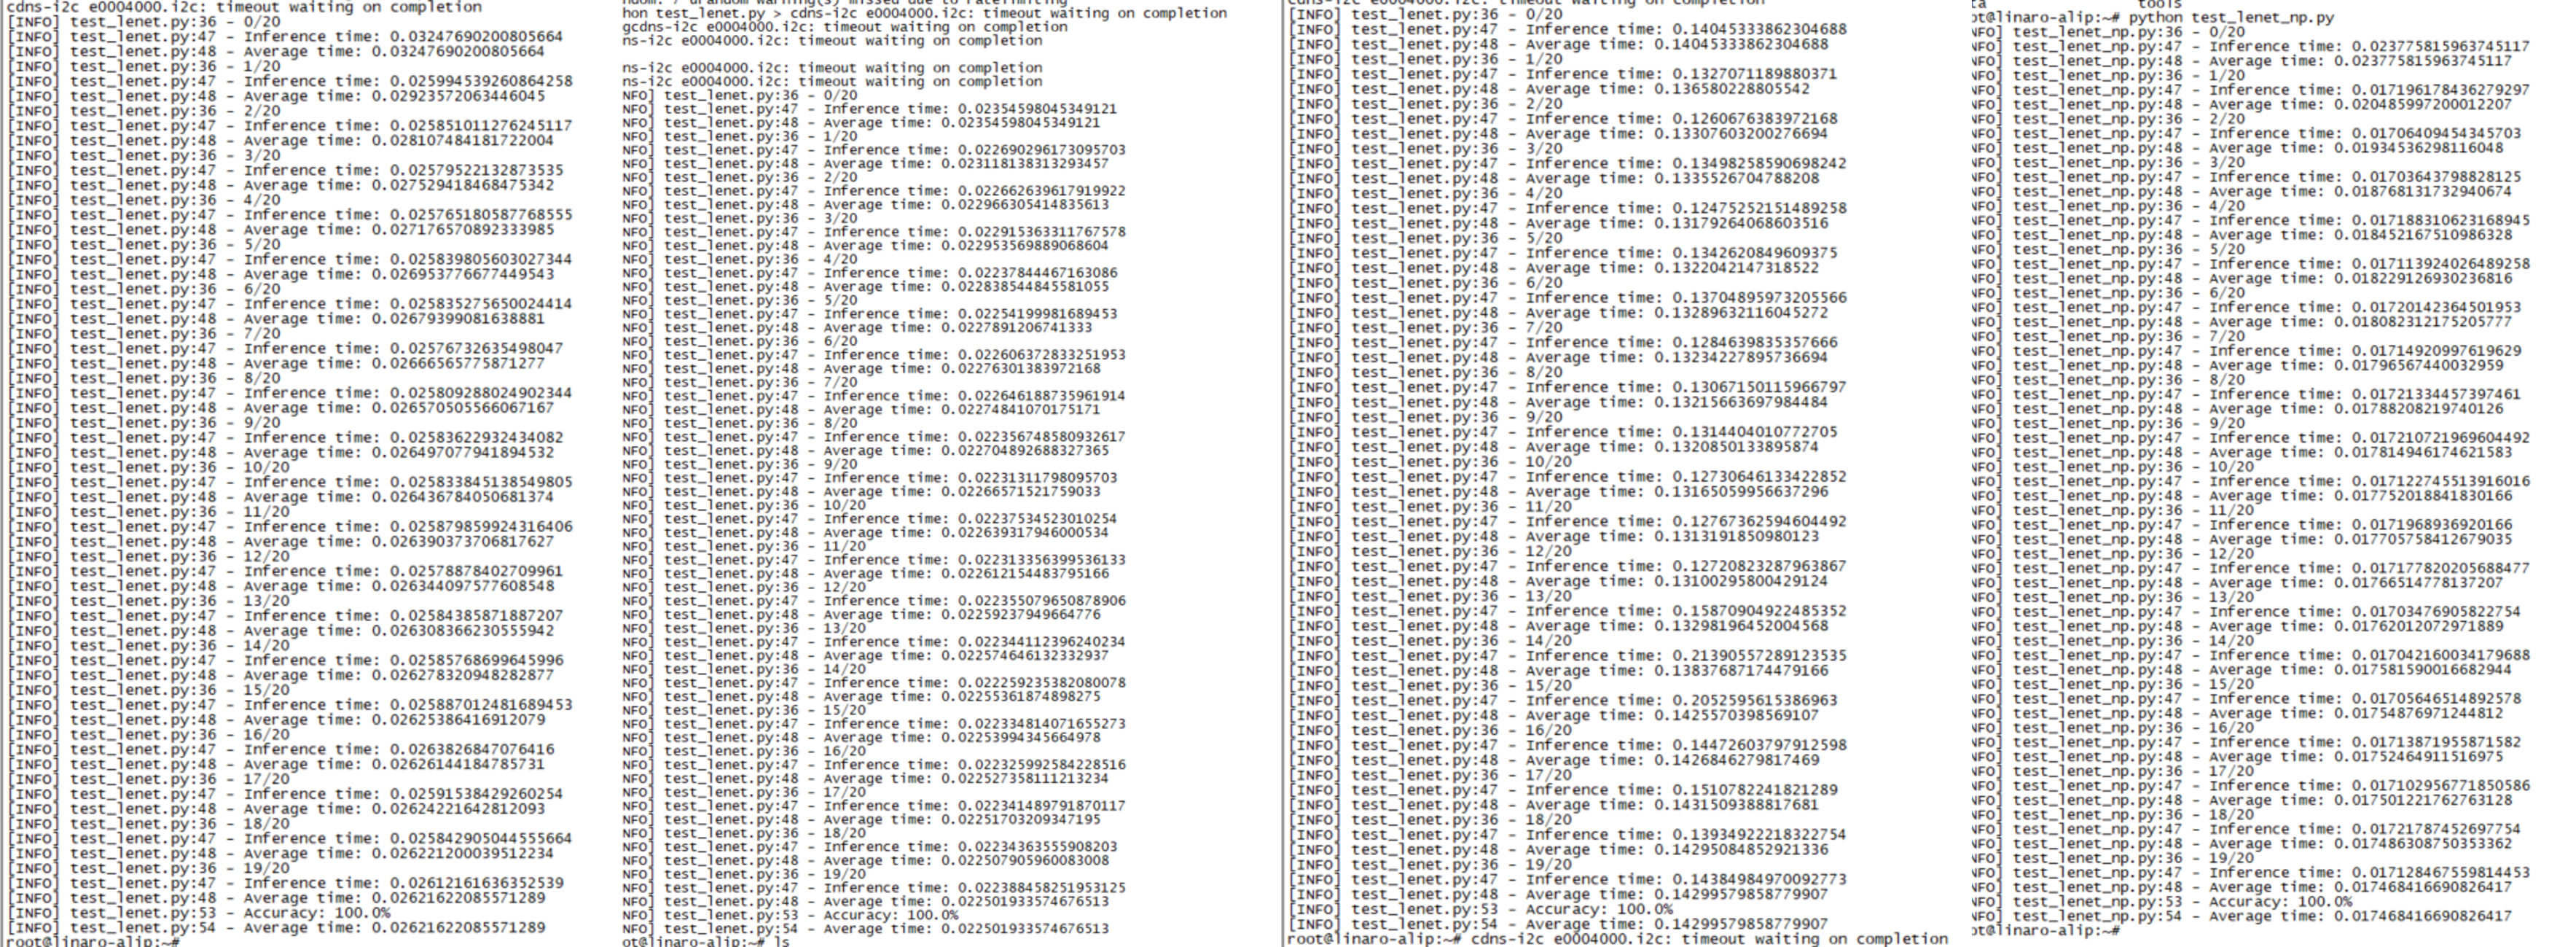
\includegraphics[width=1\linewidth]{img/lenet_time.png}
  \caption{lenet time}
\end{figure} 

MLP的运行时间:(从左到右与表格的顺序一致)

\begin{figure}[htbp]
  \centering
  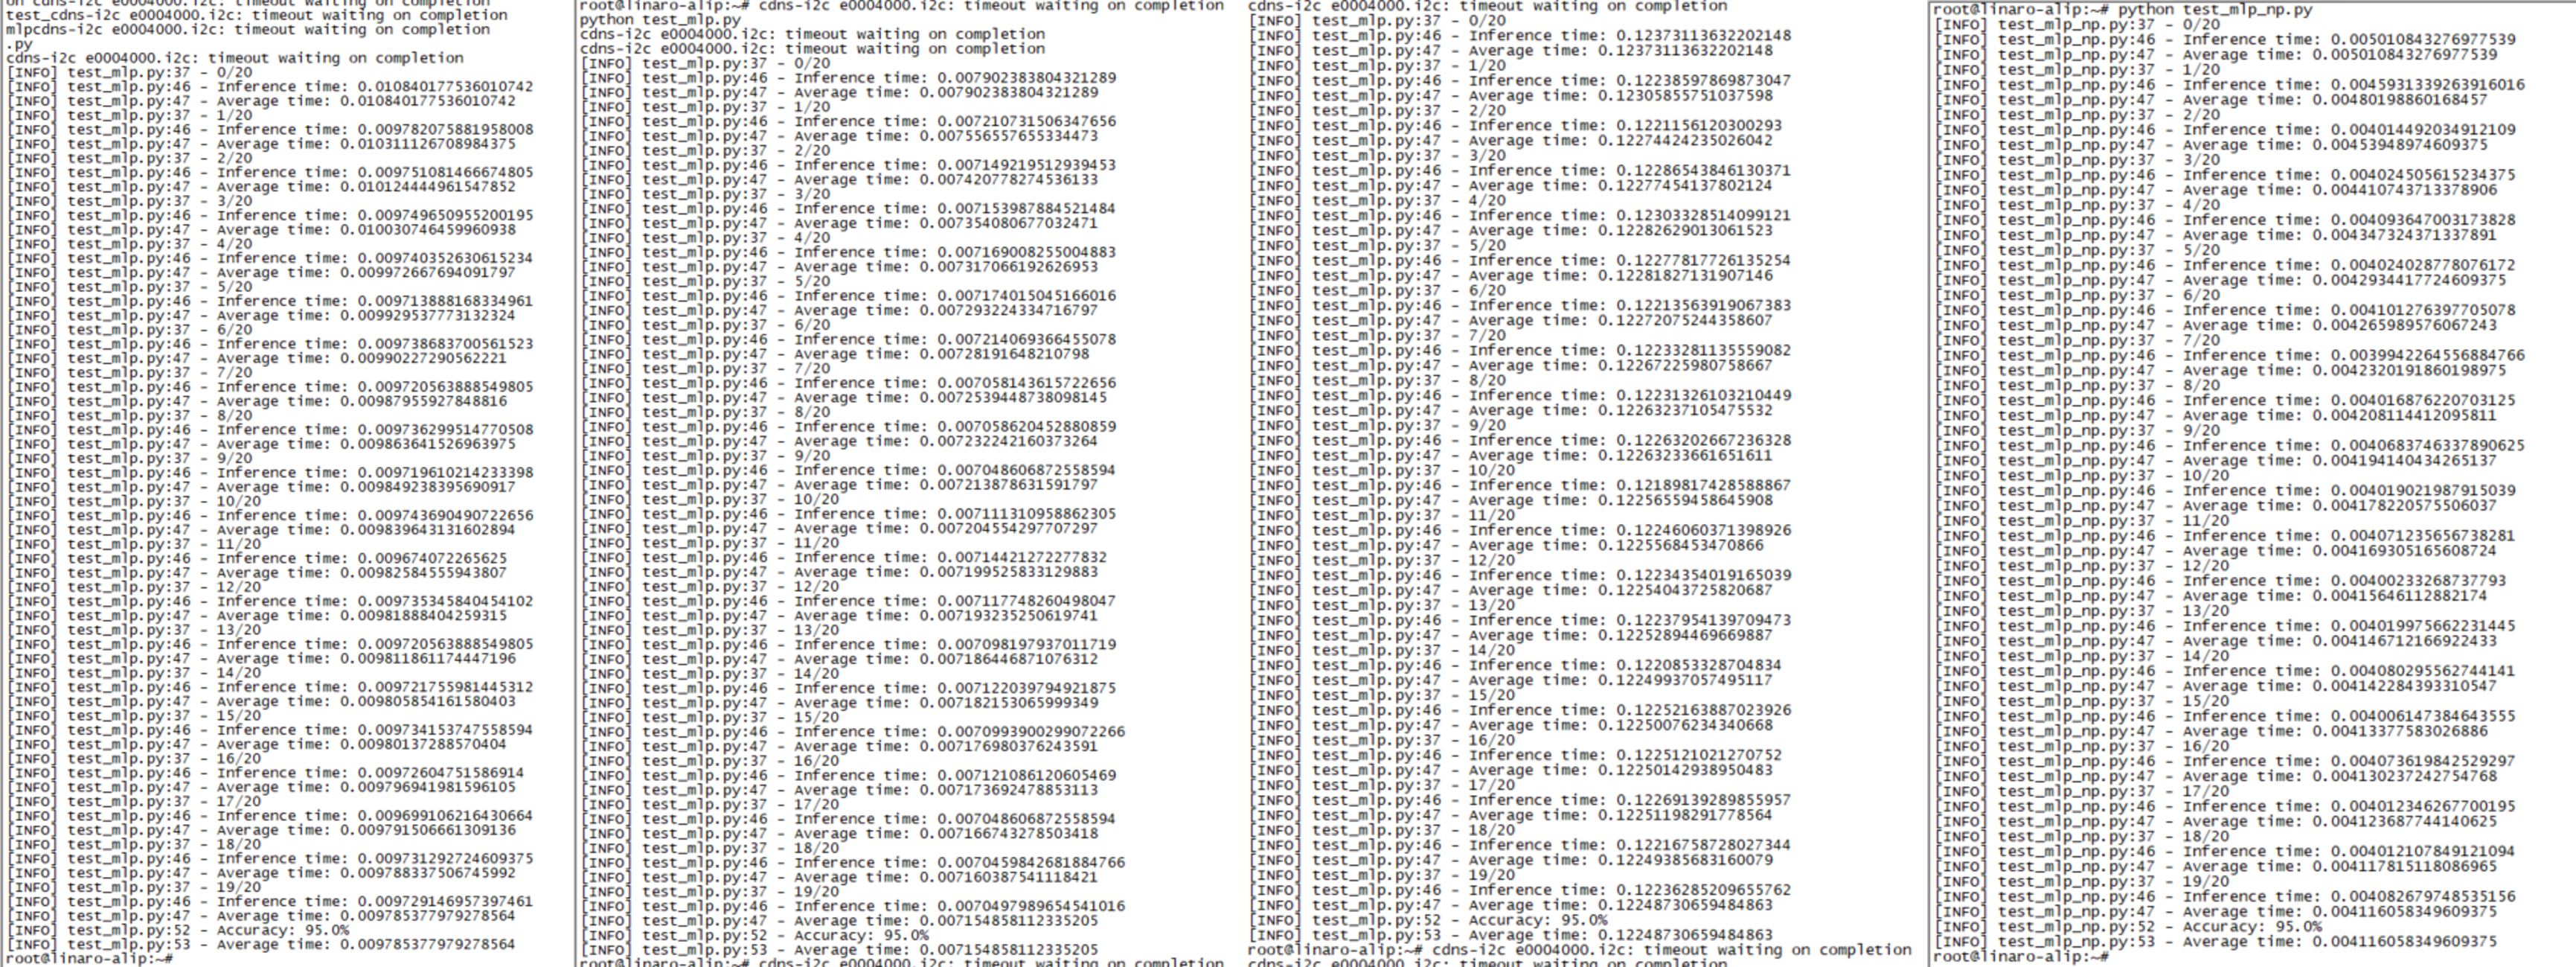
\includegraphics[width=1\linewidth]{img/mlp_time.png}
  \caption{mlp time}
\end{figure} 

\subsection{基本问题分析}

对比使用\texttt{np.matmul}和使用\texttt{matmul}的运行时间,可以得出结论:使用TPU进行计算具有一定的优化效果,但效果并不是十分显著。

分析LeNet使用的数据可以发现,所进行乘的矩阵大小基本在20*20左右,在进行矩阵运算时,会涉及到矩阵分块和频繁的数据搬运操作。在运行主频较低的FPGA上,频繁的数据搬运会成为运行的瓶颈之一。

综上,可以得到对运行时间的比对分析:

\begin{enumerate}
\item
  硬件加速:TPU的矩阵乘具有良好的加速效果,可以同时执行多个操作,这使得FPGA在执行矩阵乘法等并行度高的操作时具有天然优势。
\item
  数据搬运开销:FPGA进行矩阵乘需要频繁在FPGA侧和ARM侧进行数据搬运,每一次搬运都需要经过\textbf{发送指令-等待响应-搬运数据}的漫长流程,导致数据搬运的花销极大,与TPU带来的加速效果相抵,使得加速效果不明显
\item
  主频较低带来的影响:由于FPGA侧的主频较低(MHz),在数据传送上会使得总线的响应较慢,带来整体的数据传送速度大大降低
\item
  Zynq本身的加速效果:在ARM侧,Zynq本身的乘法器和除法器均具有本身的优化效果,使得直接使用\texttt{numpy}调用ARM测的乘法器进行矩阵乘无需经过漫长的数据搬运,可以节省大量的时间:

  \begin{itemize}
  \item
    \textbf{速度优化与面积优化}:Zynq的乘法器可以配置为速度优化或面积优化。速度优化充分利用乘法器原语,提供最高性能的实现,而面积优化则结合使用片上逻辑和专用乘法器原语,以降低基于DSP切片的乘法器利用率,同时仍能保持合理的性能。
  \item
    \textbf{DSP48E1切片}:对于乘法器尺寸不超过47x47的情况,可以选择速度优化或面积优化。对于尺寸超过47x47的乘法器,仅允许进行速度优化。
  \item
    \textbf{基于LUT的乘法器}:面积优化可以在牺牲可实现时钟频率的前提下减少延迟和LUT利用率。当两个输入操作数均为无符号数且大小均小于16位时,面积优化效果最为显著。
  \end{itemize}
\end{enumerate}

综上,可以得到分析:硬件确实有一定的加速效果,但是出于种种原因,加速效果较为一般,可以进行更多的优化。

\subsection{附加题:跳地址}

在使用跳地址后,反而出现了较为明显的\textbf{负优化},猜测结果为:跳地址过程中对数据的写为每次写一个字节,会频繁地开启BRAM,在ARM侧和FPGA侧进行频繁的数据搬运带来了巨大的时间花销。

而原先的写数据方式只需要向BRAM中发送一次数据搬运请求,可以减少数据搬运开启的时间花销,降低了不必要的损耗。

\begin{lstlisting}
# 一次只搬运一个数据带来了巨量花销
data = data.copy(order='C')
for i in range(n):
    self.bram.write(data[i], block_name=block_name, offset=i * p)
\end{lstlisting}

因为这个原因,使得FPGA的加速效果被抵消,反而取得了交叉的运行时间。

\subsection{附加题:总线位宽}

在改变总线位宽后,取得了较为显著的运行时间提升。

合理猜测原因为:数据总线的宽度提升让一次能够搬运更多的数据,节省了数据搬运的时间,让TPU的加速效果有了较为显著的提升。

\subsection{附加题:能否继续提升}

答案是:能。

当前的运行瓶颈依然在数据搬运过程,需要频繁地在FPGA侧和ARM侧进行数据搬运,有效的解决方案就是缓解这样的数据搬运花销。

下面提出了几种可行的解决方案。

\subsubsection{提升主频}

提高FPGA侧的主频,可以提高数据搬运速度,减少数据搬运带来的损耗。

提升主频可以增加总线的时钟频率,从而提高数据传输的速率。这意味着在单位时间内可以传输更多的数据,提升了总线的数据搬运能力。并且,主频的提升可以减少数据传输的延迟。在AXI等高速接口中,更高的频率意味着更低的传输延迟,这对于需要快速响应的系统尤为重要。

\subsubsection{使用乒乓模式}
当前若要进行一次矩阵乘法,就需要从cpu向矩阵乘法加速器的buffer搬运一次数据,并搬回一次,这个过程是完全串行的

可以进行一定的时间压缩,如设置不同的buffer区域,使得乘法器在运算的同时,cpu可以准备下一次运算的数据

即提升为乒乓模式。让任务在一定程度上并行,提高模块的整体吞吐量和效率

\subsubsection{使用DMA}

当前的加速模块,使用AXI-GP与PS侧通讯。但是AXI-GP的通讯效率较低,cpu将数据写入到AXI-GP需要绕过内部的Cache,写入效率也并不高。

ZYNQ实现上,为其ARM核加入了一个AXI-ACP接口,该接口直连CPU核的SCU,拥有高性能以及与CPU核心的缓存一致性。

如果在PL侧实现一个DMA,通过配置寄存器指定内存中数据的地址,由DMA将对应数据直接搬运到PL侧的bram,计算完成后再搬运回去。这样实现可以大幅度的提高PL与PS侧的通讯性能,且尽可能的使用片上的l2
cache提高性能,尽量不使io变成系统的性能瓶颈。

\subsubsection{“存算一体”扩展}

进行“存算一体”扩展:目前的计算瓶颈主要集中在\textbf{向BRAM}中搬运数据,如何节省向BRAM中搬运数据,直接在FPGA侧集成数据存储,直接利用低延迟数据传输进行计算,可以大大降低延迟,提高计算吞吐率。

可能的猜想为提高硬件上的LUT等单元,实现较好的数据存储。

\subsubsection{模型量化与剪枝}

如果硬件难以进行提高,可以考虑从软件方面进行优化。常用的手段为模型量化与剪枝:

\begin{itemize}
\item
  模型量化:这是一种通过减少模型中权重和激活函数的位宽来降低模型大小和计算复杂度的技术。量化可以将浮点数转换为低精度的表示,如从32位浮点数(FP32)转换为16位浮点数(FP16)或8位整数(INT8)。这样做不仅可以减少模型的存储需求,还可以加快推理速度,因为低精度的计算通常更快,并且对内存带宽的需求也更低。
\item
  模型剪枝:剪枝技术通过移除神经网络中的冗余或不重要的参数(如权重)来减小模型规模和提高效率。剪枝可以分为结构剪枝和非结构剪枝两种:

  \begin{itemize}
  \item
    结构剪枝:删除整个层或者一些特定的通道、滤波器等结构,这种剪枝方式能够显著减少模型的大小,但可能会影响到模型的泛化能力。
  \item
    非结构剪枝:直接删除某些权重或节点,这种剪枝方式更加灵活,但由于剪枝后的模型权重矩阵变得稀疏,可能需要特殊的硬件或软件支持才能高效运行
  \end{itemize}
\end{itemize}

目前的代码中已经实现了模型量化,利用剪枝可以进行更多的优化。

\section{实验结果与分析}

实验成功实现了在板上实现图像识别,利用FPGA上的NativeTPU单元实现硬件推理加速功能。

\begin{figure}[htbp]
  \centering
  \includegraphics[width=1\linewidth]{img/result.png}
  \caption{实验结果}
\end{figure}

综合上述实验可以得到结果:

\begin{enumerate}
\item
  TPU确实有一定的加速效果,尽管主频较低,但是依然对矩阵乘法有着加速效果
\item
  目前的瓶颈在于数据搬运,从FPGA侧到ARM侧往返搬运数据成为了瓶颈所在,需要提高数据搬运的效率
\end{enumerate}

\section{实验总结}

从一开始的CNN到如今运行在开发板上的NativeTPU,我明白了如何使用硬件,即“智能计算体系结构”来实现对“智能计算”的加速,从底层视角支撑上层的加速运算。

当下是一个大模型井喷的时代,人人渴望从软件的视角进行代码书写,使用AI来进行加速。自顶向下,大模型,LLM-serving,vllm等sys调度优化,os调度优化,到如今实现的体系结构优化。CS的世界从来不是铁板一块,而是带有着紧密串联的全体视角。

在课程开始之前,我并不知道怎么调度CPU之外的模块,以为离不开地址空间的约定、编译器的帮助,如今看着矩阵乘的输出,一种喜悦感油然而生:自顶向下,自底向上,逻辑的算符在电子中流淌,编制了智能计算的世界。

\begin{figure}[htbp]
  \centering
  \includegraphics[width=0.6\linewidth]{img/zynq.jpeg}
  \caption{zynq架构图}
\end{figure}

\end{document}
